% 前所未有简单地,开始你的 LaTeX 之旅

%%%%%%%%%%%%%%%%%%%%%%%%%%%%%%%%%%%%%%%%%%%%%%%%%%%%%%%%%%%%%%%%%%%%%%%%%
% [页面选项]
%
% 字号选项:    11pt是字号,比较适合电子印刷品和纸质印刷品
% 字体选项:    不填写 - 默认为 Modern (别忘了连逗号一起删了)
%			  times - Times New Roman
%			  sans - Sans Serif 字体(黑体)
% oneside:    代表单面,一般单侧用于电子印刷品
% 		      可以改成 twoside,一般用于双面纸质印刷
% openright:  双面打印的情况下,纸质印刷品要求新的一章从奇数页开始
% hardcopy:   打印机打印选项,带有此选项将去除logo颜色以及代码颜色,更适合黑白印刷
%			  使用彩色或者电子版请去除此选项
%			  也可以改为 editing ,颜色讲和 sublime3 的 Mariana 颜色主题一致,减小写作时的文本对比度
%		          让你以最舒适的方式书写
% heading:    页面带有页眉
\documentclass[12pt,times,oneside,openright,hardcopy]{eeereport}
%%%%%%%%%%%%%%%%%%%%%%%%%%%%%%%%%%%%%%%%%%%%%%%%%%%%%%%%%%%%%%%%%%%%%%%%%

%%%%%%%%%%%%%%%%%%%%%%%%%%%%%%%%%%%%%%%%%%%%%%%%%%%%%%%%%%%%%%%%%%%%%%%%%
% [封面选项]
%
% title:    文章主标题,不可以省略
% subtitle: 副标题,可以省略,但不可以删除
% covercontent: 封面信息,可以在其内部添加或者删除 \converline 来添加或者删除一行
%    coverline{项目}{项目内容},可以自由添加各种内容
%
\title{report title}
\subtitle{Final Thesis}

%%这里封面信息里在xjtlu_cover.tex的表格中进行更改。
%\covercontent{
%	
%	\coverline{Student Name}{Yifan Geng}
%	\coverline{Student ID}{1929573}
%	\coverline{Supervisor}{Steven Guan}
%	\coverline{Accessor}{Steven Guan}

%
%}

\begin{document}
% set line spacing to 1.5B
\baselineskip = 17pt
\pagenumbering{Alph}
\begin{titlepage}

% 不要编译!该文件已经包含在 report.tex 里了
\thispagestyle{empty}
\newcommand\nbvspace[1][3]{\vspace*{\stretch{#1}}}
\newcommand\nbstretchyspace{\spaceskip0.5em plus 0.25em minus 0.25em}
\newcommand{\nbtitlestretch}{\spaceskip0.6em}
\newcommand{\psubtitle}[1]{\Large\textbf{{#1}}\\\normalsize}
\newcommand{\ptitle}[1]{\Large\textbf{{#1}}\\\normalsize}
\newcommand{\stitle}[1]{\small\textbf{{#1}}\\\normalsize}

\begin{center}
\nbvspace[0.5]
%插入logo图片
\begin{figure}[h]
\centering
\includegraphics[width=10cm]{\logofile}
\label{fig:logo}
\end{figure}
%%%%
\psubtitle{
SCHOOL OF ADVANCED TECHNOLOGY
SAT301 FINAL YEAR PROJECT
}
\nbvspace[1]
\ptitle{\rtt}
\nbvspace[0.5]
\psubtitle{\srtt}
\nbvspace[1]
%居中
\begin{center}
\stitle{In Partial Fulfillment\\
of the Requirements for the Degree of\\
Bachelor of [Computer Science](change the phrase in [] if not applicable)}
\end{center}
\nbvspace[1]



\begin{table}[!hbp]
\centering
\begin{tabularx}{\textwidth}{|l|X|}
\hline
Student Name: &  John Doe  \\ \hline
Student ID:   &  1234567     \\ \hline
Supervisor:   &  Jane Doe \\ \hline
Assessor:     &  Jane Doe \\ \hline
\end{tabularx}

\end{table}
\normalsize
\nbvspace[0.5]

\end{center}
\newpage
\thispagestyle{empty}
\end{titlepage}

\frontmatter


	
%%%%%%%%%%%%%%%%%%%%%%%%%%%%%%%%%%%%%%%%%%%%%
% 摘要部分 Abstract/Ackowledge/
%%%%%%%%%%%%%%%%%%%%%%%%%%%%%%%%%%%%%%%%%%%%%
\mainmatter
\pagenumbering{roman}
\chapter*{Abstract}
An abstract is usually one to three paragraphs long with a length of 150 to 350 words.\\

\noindent
{\fontfamily{phv}\fontsize{11}{13.2}\selectfont \textbf{Key Words:} A maximum; of 6 words, or phrases; separated with semi-colons; no punctuation; at the end.}
\addcontentsline{toc}{chapter}{Abstract}
\chapter*{Acknowledge}
\addcontentsline{toc}{chapter}{Acknowledge}

%%%%%%%%%%%%%%%%%%%%%%%%%%%%%%%%%%%%%%%%%%%%%
%目录
%%%%%%%%%%%%%%%%%%%%%%%%%%%%%%%%%%%%%%%%%%%%%
\tableofcontents
\addcontentsline{toc}{chapter}{Contents}
\addcontentsline{toc}{chapter}{List of Figures}
\addcontentsline{toc}{chapter}{List of Tables}
\addcontentsline{toc}{chapter}{List of Acronyms}

\listoffigures   % 生成图目录
\listoftables    % 生成表目录
\chapter*{List of Acronyms}
\begin{acronym}[HTML]
\acro{HTML}{Hypertext Markup Language}
\acro{CSS}{Cascading Style Sheets}
\acro{JS}{JavaScript}
\end{acronym}

%%%%%%%%%%%%%%%%%%%%%%%%%%%%%%%%%%%%%%%%%%%%%
% 正文部分 Main Content
%%%%%%%%%%%%%%%%%%%%%%%%%%%%%%%%%%%%%%%%%%%%%
\mainmatter
\pagenumbering{arabic}


\chapter{Introduction}\label{cpt:intro}
Lorem ipsum dolor sit amet, consectetur adipiscing elit. Ut posuere, enim et blandit bibendum, ante nisl maximus nunc, sed ornare augue ante vel velit \cite{russakovsky2015imagenet}. Ut leo orci, volutpat eget ligula non, placerat elementum velit. Etiam euismod erat vel nunc blandit tincidunt. Aliquam in odio in turpis bibendum sollicitudin. Sed varius porta tempor. Proin dapibus velit vitae metus tincidunt as shown in Fig.\ref{fig:fig_example1}, sed congue magna maximus. Mauris massa risus, sodales at ligula at, suscipit vehicula odio \cite{ng2002spectral}.

\figpdf{Proin dapibus velit vitae metus tincidunt sed congue magna maximus}{fig_example1}{12cm}

Donec sapien mauris, bibendum id magna tristique, hendrerit facilisis magna. Proin ac posuere tellus, id laoreet augue. Suspendisse consequat sit amet dui in convallis \cite{einstein1935can}. Fusce tempor eros orci, eu aliquet purus placerat ut. Fusce dapibus placerat lacus ac venenatis. Etiam efficitur semper nisi lobortis vulputate. Maecenas tempor vulputate gravida. Fusce lobortis lobortis justo quis gravida. Proin tincidunt rhoncus nunc nec sodales. Phasellus ac eleifend ligula. Aliquam viverra dolor velit, quis tempor mi varius in. Aenean semper auctor nibh at consequat. Suspendisse quis fermentum enim. Cras venenatis, ligula sed convallis facilisis, augue metus vestibulum massa, nec finibus purus libero eu lacus. Aliquam finibus interdum metus, id dictum turpis. Donec erat ipsum, interdum et consequat et, vulputate convallis ante.

Integer tincidunt imperdiet iaculis. Donec pharetra neque velit, nec accumsan lorem euismod a. Etiam eget semper urna, eget porta ante. Curabitur auctor, felis id hendrerit congue, nulla sapien egestas arcu, non aliquam ante metus a elit. Nam volutpat, eros posuere facilisis malesuada, nunc tortor varius risus, sed finibus lorem lorem in ligula. Vivamus non ultrices ipsum, nec bibendum arcu. Duis ut erat lectus. Nullam vulputate purus felis. Praesent maximus laoreet eros. Duis dignissim justo odio, quis faucibus dolor tristique ac. Donec hendrerit dignissim velit sit amet tincidunt. Quisque et aliquet lorem. Integer felis felis, tempor in massa a, ultricies posuere elit. Nulla suscipit leo in justo egestas imperdiet. Nulla pharetra, dolor non volutpat tempor, ante justo luctus lectus, sit amet tincidunt elit ex ac purus.

Sed tempor ligula at maximus lacinia. Fusce vehicula velit vel sagittis rutrum. Integer quis purus quam. Vestibulum dictum, odio eu scelerisque tristique, dolor neque auctor lorem, quis auctor massa dui vitae nisi. Lorem ipsum dolor sit amet, consectetur adipiscing elit. Phasellus feugiat sit amet dolor eu ornare. Aliquam neque tellus, suscipit sed erat vitae, rutrum finibus nibh. In hac habitasse platea dictumst. Quisque malesuada dictum eros.

Etiam rhoncus tincidunt consequat. Aliquam imperdiet diam id sem condimentum condimentum. Aenean luctus egestas gravida. Duis sem risus, commodo eget facilisis at, posuere et metus. Aliquam quis tincidunt nunc. Nullam consectetur, massa id congue facilisis, dui neque lacinia orci, non vehicula nisi diam eget mauris. Praesent in laoreet nisl. Integer sodales ex in ligula sagittis, nec tincidunt velit imperdiet. Nam vulputate quis dui scelerisque rhoncus. Fusce eros erat, semper a tristique in, semper et enim. Curabitur id nisi ipsum. Morbi vitae venenatis neque. Maecenas risus odio, imperdiet ac massa vitae, ullamcorper pellentesque nunc. Curabitur auctor nunc eros, ac pulvinar lacus dictum tincidunt. Maecenas gravida non tortor ut laoreet. Curabitur mauris felis, laoreet eu volutpat et, facilisis sed elit.
\chapter{Literature Review}\label{cpt:lr}

Aenean ac pulvinar lacus, sit amet sodales lacus. Donec eu nulla lectus. Morbi ac lacus iaculis, molestie ex in, pharetra mi. Pellentesque non mattis neque. Donec auctor lacus a ligula sagittis, eu pulvinar libero pellentesque. Cras vitae sodales nulla. Curabitur risus justo, aliquam condimentum congue commodo, pellentesque vel ipsum. Cras rutrum augue quis magna vestibulum, non imperdiet neque tincidunt. Praesent at egestas nibh. Pellentesque habitant morbi tristique senectus et netus et malesuada fames ac turpis egestas.

Sed finibus molestie massa, cursus semper justo consequat in. Sed id porttitor elit. Morbi elementum finibus sollicitudin. Quisque sed molestie neque, vulputate ultrices mi. Mauris et purus libero. Nunc eu tortor vitae turpis ultricies sollicitudin. Duis justo lorem, porttitor id ipsum at, eleifend tincidunt lacus. Nullam ultrices massa vitae dui volutpat euismod. Morbi mollis porttitor nisi, eu porta orci porttitor a. Aliquam tristique, massa vel sollicitudin commodo, ligula dolor pulvinar mi, ut dictum magna risus quis libero \cite{bibname}. Vestibulum tincidunt nisi sit amet ligula placerat, eu rhoncus nibh posuere. Maecenas feugiat orci a nisl rhoncus maximus. Mauris tincidunt sodales nisl, in fermentum leo. Integer sit amet ultricies nisi. Maecenas tortor urna, vulputate ac eleifend vitae, lobortis quis erat.

Nam mauris ligula, eleifend et ipsum luctus, suscipit commodo ante. Ut sed lacinia nunc, eu dictum sapien. Etiam vehicula id lacus at ultricies. Morbi consequat vel justo nec interdum. Donec ultricies venenatis nibh nec pellentesque. Vivamus varius massa sit amet ipsum dignissim faucibus. Donec semper et nulla ornare suscipit. Suspendisse luctus malesuada bibendum. Mauris consectetur nisl quis nulla varius aliquet.

Quisque faucibus, lacus vel iaculis malesuada, nisl orci maximus erat, at sollicitudin purus dui id metus. In rhoncus urna quis risus vehicula, in eleifend enim hendrerit. Etiam fringilla lorem est. Suspendisse tincidunt malesuada interdum. Maecenas semper, sapien nec mollis pulvinar, lacus velit imperdiet ante, id tristique eros neque ut libero. Nullam pharetra odio ipsum, quis blandit magna faucibus id. Quisque sagittis nisi eget leo iaculis laoreet. Interdum et malesuada fames ac ante ipsum primis in faucibus.

Sed sapien turpis, tempor sit amet justo ut, fringilla cursus sapien. Morbi tincidunt at neque nec consequat. Praesent massa tellus, tincidunt non erat eget, posuere tristique lacus. Donec at sem vel ipsum egestas viverra. Sed id diam tincidunt, porttitor elit vel, hendrerit risus. Pellentesque dolor nibh, ullamcorper vel tristique a, faucibus sit amet est. Pellentesque habitant morbi tristique senectus et netus et malesuada fames ac turpis egestas. Pellentesque ac orci eget leo hendrerit ultrices. Ut tincidunt nulla a tempor tempor. Donec sagittis magna neque, non faucibus orci dapibus vitae. Vestibulum eget orci at risus interdum ultrices. Proin efficitur sed turpis quis convallis. Aliquam gravida viverra ligula, eget porttitor ipsum volutpat et. In sollicitudin lectus sit amet risus bibendum pellentesque. Donec quis velit imperdiet, rutrum mauris eu, malesuada mi.


\[ f(n) =
  \begin{cases}
    n/2       & \quad \text{if } n \text{ is even}\\
    -(n+1)/2  & \quad \text{if } n \text{ is odd}
  \end{cases}
\]

In mattis luctus ipsum, non molestie lectus. Sed at nisi tempus, molestie odio nec, aliquam odio. Praesent neque eros, aliquet vel diam ut, porta faucibus felis. Aliquam scelerisque dui ante, id aliquam velit elementum sit amet. Aliquam sem leo, mollis et sodales quis, viverra in nunc. Sed accumsan rhoncus cursus. Vestibulum maximus odio quis orci feugiat, vitae vehicula mi semper. Suspendisse nec sem dignissim, vestibulum turpis in, semper mi. Morbi ut rhoncus purus. Pellentesque iaculis lorem id lorem iaculis, a condimentum lectus egestas. Etiam tempor ex quis tellus bibendum, eu iaculis tellus fermentum. Duis ultricies lorem vel est mattis faucibus. Vestibulum vel purus congue, maximus ante in, euismod risus.

\chapter{Methodology}\label{cpt:method}

\section{Aenean elementum}

Praesent vehicula cursus interdum. Morbi ex elit, dignissim vel scelerisque ut, blandit mollis turpis. Praesent dictum tellus eu gravida eleifend. In ultricies neque vitae enim vulputate eleifend. Aliquam ut tristique metus. Donec ut interdum orci. Aenean elementum pretium risus, et sollicitudin ligula sollicitudin quis. Pellentesque mollis ipsum eget tempor vehicula. Phasellus nec justo nunc. Cras posuere tortor nisl, sed viverra elit faucibus ut. Etiam sed tellus posuere, gravida metus non, bibendum odio. Quisque iaculis rhoncus volutpat:
\lists{number}{
	\item Ut vitae est sed arcu euismod pulvinar nec ut ex.
	\item Aliquam sit amet quam eget felis scelerisque pellentesque vel et augue.
	\item Vivamus hendrerit diam eu orci consectetur, at eleifend nulla sodales.
	\item Proin eget eros sit amet turpis malesuada mattis vitae et dolor.
	\item Praesent in sem elementum odio iaculis sagittis in in quam.
}

Ut ultricies vestibulum ex eu tempus. Cras id ligula ligula. Integer vel congue nisi. Vestibulum ante ipsum primis in faucibus orci luctus et ultrices posuere cubilia Curae; Aliquam ac felis blandit, porta quam ut, scelerisque nisi. Suspendisse a enim sed leo vestibulum tincidunt in vestibulum nulla. Proin suscipit ultricies magna sed fermentum. Vestibulum ullamcorper auctor lobortis. Nunc nunc nisi, facilisis a ullamcorper a, venenatis non metus. Pellentesque vel tempus massa. Morbi sed nisi lacus. Nulla lacinia urna quis placerat consequat. Quisque risus justo, rhoncus vitae nulla sed, laoreet lobortis velit.

\section{Etiam vel quam in justo}

Ut ac tortor eget magna gravida mollis sit amet ac felis. Sed id massa sit amet dui faucibus egestas vitae ac turpis. Suspendisse neque ligula, consequat eget nisi eu, ultricies hendrerit metus. Etiam felis augue, euismod eget aliquet non, gravida id justo. Etiam vel quam in justo finibus aliquet. Etiam blandit viverra felis, sed convallis urna viverra a. Nulla non volutpat ex. Curabitur ac mauris varius, dictum sapien sit amet, placerat sem:
\begin{equation}
R_T=V_T/I(\Omega)
\end{equation}

\begin{table}[h]
\label{tab:tab1}
\centering
\caption{ Title Of Table }
\renewcommand{\arraystretch}{2}
\setlength{\tabcolsep}{10pt}
\begin{tabular}{ |>{\itshape}c|p{2cm}| >{\bfseries}m{3cm}<{\centering}| }
\hline % 绘制横向表格线,在LaTeX中需要自己定义每一行的表格线
cell 11 & cell 12 & cell 13   \\
\hline
cell 21 & cell 22 & cell 23 \\
\cline{1-2}
cell 31 & cell 32 \newline 456& cell 33  \\
\hline
\end{tabular}
\end{table}

Etiam non semper elit. Vestibulum lectus enim, efficitur at malesuada non, aliquet nec ante. Pellentesque habitant morbi tristique senectus et netus et malesuada fames ac turpis egestas. Maecenas erat dolor, euismod euismod ligula at, finibus tristique sem. Aliquam ornare facilisis diam. Sed pharetra nisi nec felis finibus, a maximus lectus elementum. Proin imperdiet condimentum mi, a imperdiet ligula rutrum eget. Sed ut semper justo.

Maecenas efficitur non neque at hendrerit. Nulla vestibulum posuere interdum. Morbi eleifend tellus at eros vulputate vulputate. Etiam eget suscipit risus. In ornare ullamcorper odio vitae scelerisque. Fusce neque dolor, facilisis vitae odio sit amet, accumsan volutpat eros. Class aptent taciti sociosqu ad litora torquent per conubia nostra, per inceptos himenaeos. Maecenas sed mauris metus. In imperdiet mauris eros, vel imperdiet erat lobortis non.

Sed pretium bibendum auctor. Nam placerat semper luctus. Cras eget pretium erat. Curabitur nec venenatis felis. Etiam accumsan volutpat purus, vel scelerisque risus pulvinar et. Pellentesque eget nibh imperdiet, venenatis turpis quis, posuere dolor. Etiam quis enim in nisi cursus vulputate vitae imperdiet est. Ut vulputate orci nisi, nec pulvinar nibh porta vitae. Mauris dolor libero, gravida a aliquet in, efficitur ac eros. Maecenas vel molestie est. In convallis finibus velit, ac eleifend felis varius nec. Proin velit ex, fermentum at ligula at, scelerisque tempus eros. Lorem ipsum dolor sit amet, consectetur adipiscing elit. Nullam quis nibh felis. Lorem ipsum dolor sit amet, consectetur adipiscing elit.
\lists{dot}{
	\item Ut vel felis pellentesque, lobortis quam quis, viverra nibh.
	\item Integer commodo odio sed augue faucibus, non sodales quam sagittis.
	\item In eleifend metus eu dui iaculis mollis ut sed magna.
}

Mauris ac nisi in orci tempus consectetur lobortis nec neque. Aliquam aliquet libero lacus, sed dictum elit gravida nec. Curabitur posuere odio vel consectetur scelerisque. Proin eu augue sem. Donec faucibus mollis nisi sed placerat. Vestibulum pharetra mauris nulla, id viverra arcu scelerisque nec. Ut imperdiet metus nec ultricies consectetur. Cras ac mauris consequat, varius est at, ultrices nibh. Mauris quis condimentum nibh. Pellentesque sit amet arcu sodales, convallis diam vel, pellentesque lacus. Vestibulum ante ipsum primis in faucibus orci luctus et ultrices posuere cubilia Curae; Aenean sodales felis ac neque iaculis, non scelerisque magna congue. Praesent dignissim ultrices odio non laoreet. Aliquam et dolor tellus. Lorem ipsum dolor sit amet, consectetur adipiscing elit. Donec erat ipsum, maximus finibus auctor vel, semper in velit.
\begin{eqnarray}
\nabla\cdot\vec{E} &=& \frac{\rho}{\epsilon_0} \\
\nabla\cdot\vec{B} &=& 0 \\
\nabla\times\vec{E} &=& -\frac{\partial B}{\partial t} \\
\nabla\times\vec{B} &=& \mu_0\left(\vec{J}+\epsilon_0\frac{\partial E}{\partial t} \right)
\end{eqnarray}


\subsection{Nullam porttitor}

Nullam porttitor nunc et euismod congue. Praesent blandit ex et congue fermentum. Nullam diam velit, facilisis vel libero in, molestie vestibulum risus. Phasellus fringilla sagittis elementum. Cras malesuada odio et porta blandit. Praesent fermentum egestas arcu ut lobortis. Praesent et nunc mollis, malesuada enim eu, ullamcorper nisi. Aliquam vel pellentesque nibh, vel volutpat justo. Phasellus vitae efficitur est. Vestibulum ante ipsum primis in faucibus orci luctus et ultrices posuere cubilia Curae; Phasellus congue sapien purus, in convallis turpis sollicitudin ut. Aliquam sagittis luctus erat, sit amet dignissim tellus tristique ac. Nam auctor egestas erat a finibus. Donec fringilla ac lorem id pulvinar.

\subsection{Nulla facilisi}

Nulla facilisi. Lorem ipsum dolor sit amet, consectetur adipiscing elit. Interdum et malesuada fames ac ante ipsum primis in faucibus. Integer id malesuada nibh, id pulvinar purus. Proin non dui nec diam convallis egestas quis vel est. Pellentesque sed sem metus. Nulla placerat laoreet lorem eu venenatis. In hac habitasse platea dictumst. Morbi ut metus nulla. Duis sit amet justo dapibus, blandit libero et, vehicula diam. Class aptent taciti sociosqu ad litora torquent per conubia nostra, per inceptos himenaeos.

\section{Suspendisse}

Suspendisse dictum lectus a nulla scelerisque, pulvinar varius magna sollicitudin. Praesent sed tincidunt ligula. Ut semper vel neque quis vehicula. Interdum et malesuada fames ac ante ipsum primis in faucibus. Sed et tempus sem. Nulla id mi cursus, pretium lacus eget, malesuada velit. Cras sodales, ex et tempor mollis, diam enim sagittis nibh, at hendrerit ante ex vitae ex. Integer ipsum mi, pellentesque at metus suscipit, rutrum dignissim leo. Etiam elementum ante in ultrices interdum. Etiam faucibus neque eget odio tristique lacinia. Curabitur imperdiet ullamcorper ipsum vel tincidunt. Integer laoreet pellentesque volutpat. Praesent mauris quam, scelerisque et dictum et, mollis eget mi.


\chapter{Experiment}\label{cpt:exp}

\section{Result ante}

Donec porttitor tempor dui, ut aliquet dui ultrices sed. Nunc malesuada in Fig.\ref{fig:result1}, tellus quis efficitur dignissim, ante dui viverra diam, sit amet porta velit est vitae quam. Sed odio elit, sagittis a tellus id, rhoncus maximus augue. Donec consectetur nisi sit amet ante venenatis dictum. Nam sit amet cursus augue, quis maximus lacus. Nulla rhoncus egestas erat, vel consectetur nisl ornare ac. Pellentesque habitant morbi tristique senectus et netus et malesuada fames ac turpis egestas. Fusce rutrum imperdiet hendrerit. Aenean eu lobortis metus. Vestibulum fermentum, lacus nec euismod viverra, enim sem auctor turpis, eget tincidunt nisl augue sed elit.

\figpdf{Experimental result 1}{result1}{11cm}

\section{Result blandit}

Aenean ultrices felis ante, in neque dictum ut. Class aptent taciti sociosqu ad litora torquent per conubia nostra, per inceptos himenaeos. Vestibulum ante ipsum primis in faucibus orci luctus et ultrices posuere cubilia Curae; Maecenas porta ex quis erat egestas condimentum. Donec suscipit semper egestas. Vestibulum id massa aliquet, ullamcorper nibh vel, porttitor leo. Cras porta leo et diam tincidunt, ut viverra metus varius \Fig{result2}.

\figpdf{Experimental result 2}{result2}{9cm}

\section{Result curabitur}

In Fig.\ref{fig:result2}, curabitur consequat sodales ligula in condimentum. Praesent imperdiet, nulla eu egestas ultrices, diam elit fringilla purus, sit amet elementum lacus mauris vitae turpis. Nunc lobortis viverra est, vel porttitor orci eleifend ac. Vestibulum lacus ante, finibus a est id, ornare viverra orci. Pellentesque habitant morbi tristique senectus et netus et malesuada fames ac turpis egestas. Nam ultricies, ligula a ultrices eleifend, mi lectus interdum leo, sit amet fringilla nisi odio sit amet lectus. Nam cursus eros a mi vestibulum, sit amet lobortis lacus consectetur.



\begin{figure}[htp] %htp用来表示图片的位置
\centering 
  \subfigure[Description 1]{ 
    \label{fig:subfig:a} % 第1幅图的的标签
    % 第1幅图片的尺寸和地址
    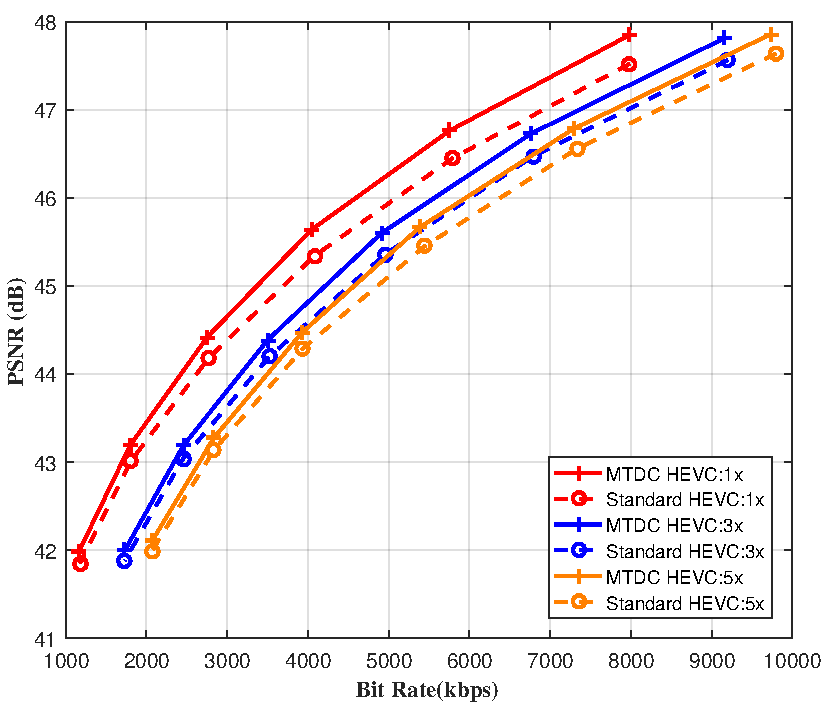
\includegraphics[width=6cm]{fig/sub1.pdf}}
  \hspace{0.5cm} % 图片的水平间隔
  \subfigure[Description 2]{ 
    \label{fig:subfig:b} % 第2幅图的的标签 
    % 第1幅图片的尺寸和地址
    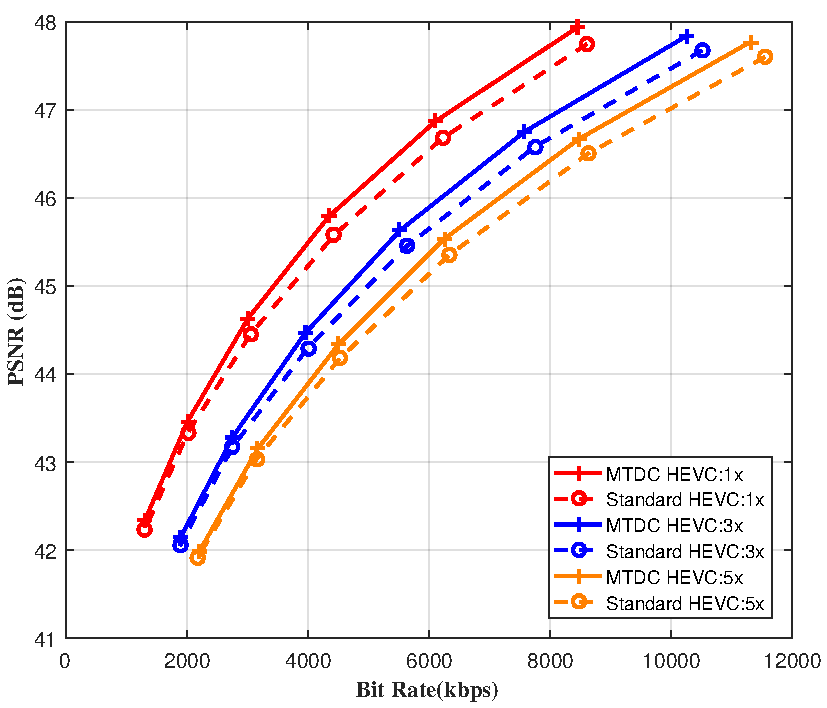
\includegraphics[width=6cm]{fig/sub2.pdf}} 
  \\ % 强制换行
  \vspace{0.5cm} % 图片的垂直间隔
  \subfigure[Description 3]{ 
    \label{fig:subfig:c} % 第3幅图的的标签
    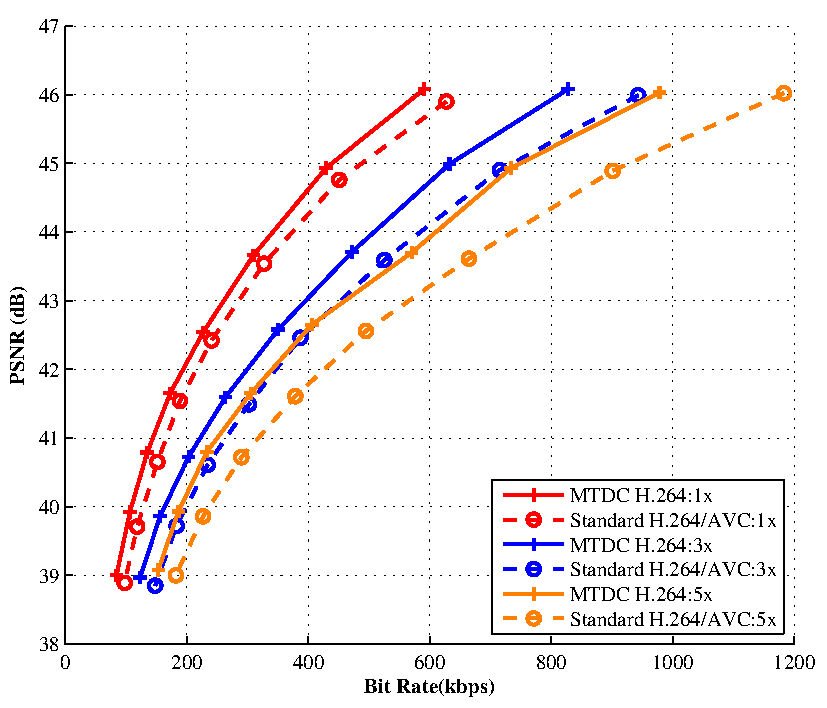
\includegraphics[width=6cm]{fig/sub3.pdf}} 
  \hspace{0.5cm} % 图片的水平间隔
  \subfigure[Description 4]{ 
    \label{fig:subfig:d} % 第4幅图的的标签
    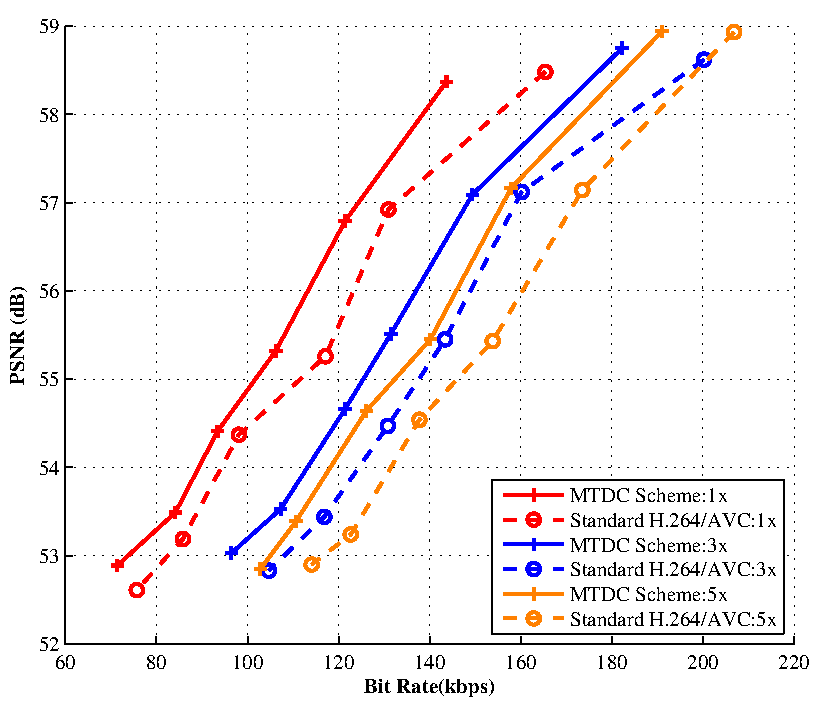
\includegraphics[width=6cm]{fig/sub4.pdf}} 
  \caption{For sub firgures located in a $2\times 2$ array} 
  \label{fig:subfig} %% label for entire figure 
\end{figure}

\begin{table}[h]
\label{tab:tab2}
\centering
\caption{ Title Of Table }
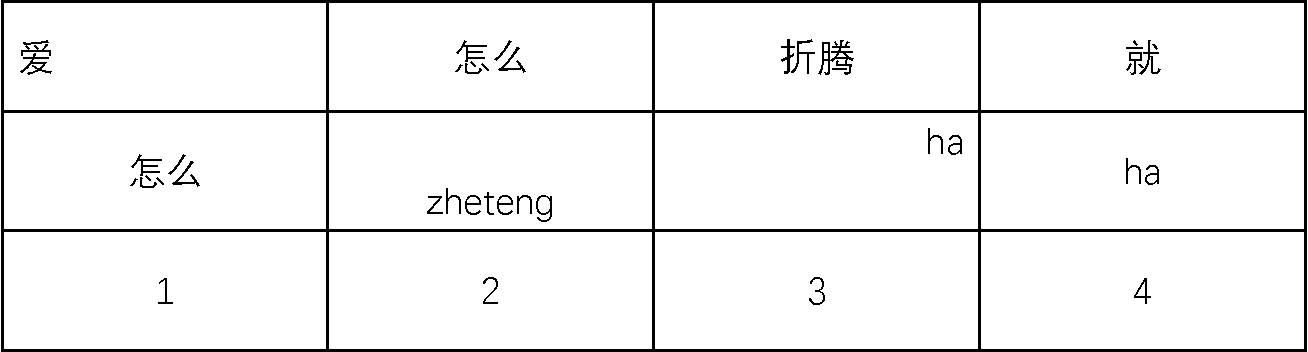
\includegraphics[width=10cm]{fig/table.pdf}
\end{table}

Sed at leo eleifend ante dapibus sollicitudin. Donec eget turpis massa. Fusce efficitur, sem eu sollicitudin rhoncus, eros nulla aliquet arcu, ut pellentesque lacus metus eu turpis. Duis venenatis eleifend leo, non lobortis tortor dictum sed. Cras eu dui quis dolor scelerisque eleifend sit amet a nibh. Suspendisse porttitor sit amet nunc sit amet hendrerit. Fusce tempus purus metus, rhoncus dictum nisl pretium vitae. Suspendisse sodales nunc velit, ac malesuada diam commodo sed. Sed maximus vel risus quis laoreet. Ut ullamcorper ante non faucibus imperdiet. Cras tristique nec ligula id egestas. Duis ut elit id lorem sodales viverra eu ut leo in Equ.\ref{equ:equation1}.

\begin{equation}\label{equ:equation1}
R^m_T=R_{180\Omega}+R_{100\Omega}+R_{120\Omega}
\end{equation}

%见到的令你感动的代码插入功能,将c代码加入到
%\code{c++}{c_test.c}

\chapter{Conclusion}\label{cpt:con}

Phasellus non rutrum quam. Curabitur et dolor in augue faucibus iaculis finibus vitae eros. Morbi fringilla ligula libero, in fringilla ipsum ultricies nec. Donec a dapibus turpis. Cras vestibulum tortor purus, vel volutpat eros interdum et. Nullam id sollicitudin ex, placerat aliquam justo. Sed finibus varius mi vehicula pulvinar. Mauris ut lacus dolor. Vivamus condimentum urna eu nunc egestas, id tempor enim vulputate. Mauris hendrerit condimentum sodales. Aenean consectetur magna sed ante tincidunt, vel tincidunt risus scelerisque. Praesent ut maximus tortor. Proin enim purus, egestas elementum mi nec, pulvinar fermentum risus. Ut id tristique justo, sit amet vehicula ante.

Vestibulum eu faucibus purus, nec consequat felis. Mauris massa nisl, sollicitudin eu luctus sed, porttitor a eros. Ut tincidunt sem vitae lacus fringilla aliquet. Lorem ipsum dolor sit amet, consectetur adipiscing elit. Pellentesque fermentum tristique mollis. Vivamus elementum pretium ante, vel mollis tellus luctus vitae. Nullam varius tristique turpis, eget mollis dui sagittis quis. Ut nec efficitur nibh.



% 参考文献列表,请打开 reference.bib 文件添加 bibtex 格式的参考文献
\bibliographystyle{IEEEtran}
\bibliography{reference} %
\addcontentsline{toc}{chapter}{References}

\chapter{Title of Appendix 1}
\label{ch:Title of Appendix 1}

\section{Appendix Heading 1}
\figpdf{Experimental result 2}{result2}{9cm}
\section{Appendix Heading 2}
Text of the appendix goes here

\section{Appendix Table and Figure Captions}
In appendices, table and figure caption labels and numbers are typed in manually (e.g., Table A1, Table A2, etc.). These do not get generated into the lists that appear after the Table of Contents. 

\chapter{Title of Appendix 2}
\label{ch:Title of Appendix 2}
Text of the appendix goes here if there is only a single heading. 
\addcontentsline{toc}{chapter}{Appendix}
\end{document}

